\documentclass[11pt,a4paper,utf8x]{article}
\usepackage{lmodern}
\usepackage[T1]{fontenc} 
\usepackage[utf8]{inputenc}  
\usepackage [frenchb]{babel}

% Pour pouvoir utiliser le verbatim dans les sections utiliser la commande versalitas
\newcommand{\versalitas}[1]{{\usefont{T1}{cmr}{bx}{sc}#1}}% 

\usepackage{textcomp}
\usepackage{keystroke}
\usepackage{amssymb}
 
\usepackage{amsmath}
\renewcommand{\thesection}{\arabic{section}} % numérotation des sectiosn
\usepackage[cc]{titlepic} %rajouter le logo dans la page de garde
\usepackage{url} % Pour avoir de belles url
\usepackage {geometry}
\usepackage[linktocpage]{hyperref}

%enlever le numéro de page
\usepackage{nopageno}
% Pour mettre du code source
\usepackage {listings}
% Pour pouvoir passer en paysage
\usepackage{lscape}	

% Pour pouvoir faire plusieurs colonnes
\usepackage {multicol}

% POur crééer un index
\usepackage{makeidx}

\usepackage[pdftex]{graphicx}

\hypersetup{
backref=true,
%permet d'ajouter des liens dans...
pagebackref=true,%...les bibliographies
hyperindex=true, %ajoute des liens dans les index.
colorlinks=true, %colorise les liens
breaklinks=true, %permet le retour à la ligne dans les liens trop longs
urlcolor= blue, %couleur des hyperliens
citecolor=	cyan,
bookmarks=true, %créé des signets pour Acrobat
bookmarksopen=true,
%si les signets Acrobat sont créés,
%les afficher complètement.
pdftitle={Services M2 ALMA}, %informations apparaissant dans
pdfauthor={MARGUERITE Alain\\ RINCE Romain},
%dans les informations du document
pdfsubject={Doc}
%sous Acrobat.
}
\hyphenation{si-tu-a-tion}
\makeindex


%%%% debut macro pour enlever le nom chapitre %%%%
% \makeatletter
% \def\@makechapterhead#1{%
%   \vspace*{50\p@}%
%   {\parindent \z@ \raggedright \normalfont
%     \interlinepenalty\@M
%     \ifnum \c@secnumdepth >\m@ne
%         \Huge\bfseries \thechapter\quad
%     \fi
%     \Huge \bfseries #1\par\nobreak
%     \vskip 40\p@
%   }}
% 
% \def\@makeschapterhead#1{%
%   \vspace*{50\p@}%
%   {\parindent \z@ \raggedright
%     \normalfont
%     \interlinepenalty\@M
%     \Huge \bfseries  #1\par\nobreak
%     \vskip 40\p@
%   }}
% \makeatother
%%%% fin macro %%%%

%Couverture 

%Couverture 
\widowpenalty=10000
\clubpenalty=10000
 
 \title{{\large \textbf{Résumé d'article}\\\emph{Agility and Architecture—Can they coexist?}\\\vspace{1ex}
 {\scriptsize Philippe \textsc{Kruchten}\\\vspace{0.5ex}University of British Columbia\\\vspace{-4ex}
Vancouver BC, Canada}}}
%\titlepic{
\includegraphics[scale=0.80]{img/logouniv}}
		

\author{\small Alain \textsc{Marguerite} et Romain \textsc{Rincé}\\{\small Encadrant : Dalila \textsc{Tamzalit}}}
\date{}
 
%\title{{\Huge Formal Software Engineering}\\{\small Encadrant : Christian \textsc{Attiogbé}}\\\vspace{3cm} Résumé d'article :\\\vspace{0.3cm}{\Large \emph{Applying Event and Machine Decomposition to a Flash-Based Filestore in Event-B}}\\\vspace{0.3cm}
%\small K. \textsc{Damchoom} and M. \textsc{Butler}\\University of Southampton\\\vspace{2cm}}
%\titlepic{
\includegraphics[scale=0.80]{img/logouniv}}
		

%\author{\vspace{2cm}Romain \textsc{Rincé}}
%\date{\small Université de Nantes \\ 2 rue de la Houssinière, BP92208, F-44322 \textsc{Nantes} cedex 03, \textsc{France}}

\hyphenation{appar-tiennent}
\hyphenation{pro-blèmes}

\begin{document}

\maketitle
\renewcommand{\labelitemi}{$\bullet$} 

\abstract{Dans le cadre de la 2\up{ème} année Master ALMA, le module \emph{Services} nous donne l'opportunité d'étudier les architectures distribuée telle que SOA (..), ainsi que des techniques de développement comme les méthodes agiles. Le but de ce document est de proposer le point de vue de notre bînome sur les méthodes agiles et l'architecture SOA. Dans la section \ref{sec:res} de ce document, nous proposons une critique d'un article de P. \textsc{Kruchten} consacrée à la coexistence entre les architectures logicielles et les méthodes agiles. Par la suite, la section \ref{sec:cri} contient le point de vue de notre bînome de l'article de P. \textsc{Kruchten}. Enfin dans l'ultime section \ref{sec:ret} nous reviendrons sur les notions étudiées proposant un nouveau point de vue.} 

\section{Résumé de l'article}\label{sec:res}
L'objectif de l'article \emph{Agility and Architecture—Can they coexist?}  \cite{krutchen} est de montrer la dichotomie qui existe entre les méthodes agiles et le développement reposant sur une architecture définie, puis de chercher une possible coexistence de ces deux concepts. 

Dans un premier temps, l'auteur tente de nous monter que les méthodes agiles ne peuvent être la solution à tout, notamment en présentant un cas où l'orientation agile d'un projet s'est conclue par un échec. 

L'auteur met en évidence que le \og niveau\fg{} d'architecture dépend des besoins spécifiques au projet et spécifie huit facteurs qui doivent être pris en compte dans la réalisation d'un projet tel que la taille ou la criticité du projet.

\section{Critique de l'article}\label{sec:cri}


\section{Retour sur l'agilité et SOA}\label{sec:ret}
Les méthodes agiles sont un ensemble de méthodes caractéristiques du développement en informatique et de la conception de logiciels. Avec la volonté d'être le plus pragmatique possible, les méthodes agiles font intervenir au maximum le client (le \og demandeur \fg{}), ce qui permet une grande réactivité à ses exigences. Le but principal étant d'être au plus près de la satisfaction réelle du client.

Une architecture orientée services (Service Oriented Architecture, SOA) est une formes d'architectures mettant en oeuvre un modèle d'interaction applicatif. Ces interactions sont possibles grâce à un ensemble de fonctionnalités basique appellées services. Ces services sont fournis par des composants (composants logiciels). On retrouve dans la référence \cite{soa} une description des nombreux avantages que propose l'architecture SOA.


Parmi eux, la modularité de ce type d'architecture permet de remplacer facilement un composant ou service par un autre. La mise à disposition des solutions au clients est donc plus rapide et moins onéreuse. Cette réduction du \emph{Time to Market} donne un avantage non négligeable à l'architecte de l'application qui peut alors trouver les moyens de créer de nouvelles fonctionalités ou simplement d'investir dans d'autre projet.


Cependant, pour être bénéfique, l'utilisation d'une architecture SOA demande certains pré-requis (\textit{cf.} \cite{soa}). Par exemple, il n'est pas raisonable d'employer une telle architecture dans le cadre d'une petite application où une architecture plus simple et plus économique à mettre en place serait suffisante. De plus, certaines pré-conditions sont indispensables pour rendre l'utlisation d'une architecture SOA pertinente (qualification des développeurs, réutilisation des servives\dots).


La référence \cite{ibm} met en exergue les conditions dans lequelles une collaboration entre SOA et méthodes agiles semble pertinente. Les architectures SOA créent naturellement des inter dépendances entre applications. Il n'existent pas, en effet d'applications SOA \og indépendantes \fg{}. De plus chaque service d'une pplication SOA doit être considéré comme un composant \og ré-utilisable \fg{}. Ces deux dernières contraintes précédement décrites impliquent un nombre de changements potentiellement important sur des intervalles de temps réguliers. Dans un tel contexte, l'utilisation de l'agilité semble raisonable.  



% \begin{figure}[htbp] %on ouvre l'environnement figure
%   \center
%   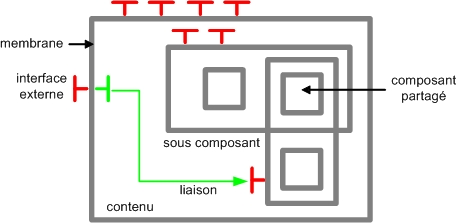
\includegraphics{img/fractal_component}
%   \caption{Exemple d'un modèle \fractal{} de composants} %la légende
%  \label{fig:Comp} %la légende
% \end{figure}


 %on ferme l'environnement figure
% Pour avoir un interligne de 1,5
% \input{P0}
%\input{P01}
% \input{P1}
% \input{P2}
% \input{annexereal}

% Pour finir l'interligne de 1,5

% \printindex
% 
% \appendix
\bibliographystyle{alpha}
\bibliography{biblio.bib}

\end{document}

%%  LocalWords:  Master ALMA SOA bînome Krutchen Agility Can they
%%  LocalWords:  coexist criticité Oriented
